\documentclass{beamer}

\usepackage[utf8]{inputenc}
\usepackage{default}
\usepackage{amssymb,amsmath,amsfonts}
\usepackage{graphicx}
\usepackage{color}
\usepackage{subcaption}
%\usepackage{colortbl}
%\usepackage{todonotes}
\usepackage{hyperref}
\usepackage{cleveref}
%\usepackage{subfig}
\usepackage{bm}
%\usepackage{listings}
\usepackage{multimedia}
%\usepackage{media9}
%\usepackage{multirow}
%\usepackage{cite}
\usepackage[round]{natbib}   % omit 'round' option if you prefer square brackets
\bibliographystyle{plainnat}

\mode<presentation>
{
    \usetheme{Madrid}
    \usecolortheme{rose}
}


\newcommand{\highlight}[1]{%
  \colorbox{red!50}{$\displaystyle#1$}}
  
  \newcommand{\x}{\mathbf{x}}
\newcommand{\y}{\mathbf{y}}
\newcommand{\q}{\boldsymbol{\theta}}
\newcommand{\io}{\int_\Omega}
\newcommand{\ve}{\varepsilon}
\newcommand{\pa}{\partial}

\newcommand{\F}{\mathbf{F}}

\newcommand{\highlightcustom}[2][yellow]{\mathchoice%
  {\colorbox{#1}{$\displaystyle#2$}}%
  {\colorbox{#1}{$\textstyle#2$}}%
  {\colorbox{#1}{$\scriptstyle#2$}}%
  {\colorbox{#1}{$\scriptscriptstyle#2$}}}%

  
\setbeamertemplate{headline}{%
    \leavevmode%
    \hbox{%
        \begin{beamercolorbox}[wd=\paperwidth,ht=2.5ex,dp=1.125ex]{palette quaternary}%
            \insertsectionnavigationhorizontal{\paperwidth}{}{\hskip0pt plus1filll}
        \end{beamercolorbox}%
    }
}


\title[Scalar Reduction of a Neural Field]{Scalar Reduction of a Neural Field Model with Spike Frequency Adaptation} % The short title appears at the bottom of every slide, the full title is only on the title page

\author[Y. Park \& G.B. Ermentrout]{Youngmin Park \& Bard Ermentrout} % Your name
\institute[U Pitt]% Your institution as it will appear on the bottom of every slide, may be shorthand to save space
{
University of Pittsburgh Department of Mathematics\\ % Your institution for the title page
\medskip
\textit{yop6@pitt.edu} % Your email address
}
\date{\today} % Date, can be changed to a custom date

% show page number
\addtobeamertemplate{navigation symbols}{}{%
    \usebeamerfont{footline}%
    \usebeamercolor[fg]{footline}%
    \hspace{1em}%
    \insertframenumber/\inserttotalframenumber
}

\begin{document}

\begin{frame}
\centering
\includegraphics[width=.2\textwidth]{pitt.png}
\titlepage % Print the title page as the first slide
\end{frame}
% 
% \begin{frame}
% \frametitle{Overview} % Table of contents slide, comment this block out to remove it
% \tableofcontents % Throughout your presentation, if you choose to use \section{} and \subsection{} commands, these will automatically be printed on this slide as an overview of your presentation
% \end{frame}

%\begin{frame}
%\frametitle{Overview} % Table of contents slide, comment this block out to remove it
%\tableofcontents % Throughout your presentation, if you choose to use \section{} and \subsection{} commands, these will automatically be printed on this slide as an overview of your presentation
%\end{frame}

\begin{frame}
 \tableofcontents
\end{frame}



\section{Introduction (Modeling)}
\subsection{Short Term Memory Task}
\begin{frame}
\frametitle{Introduction: T-Maze Task Decision}
\begin{figure}
 \centering
 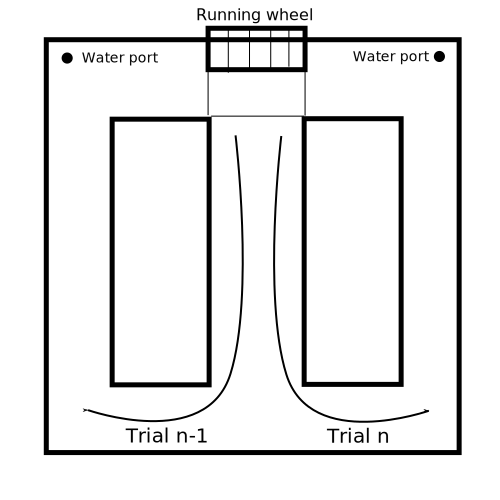
\includegraphics[width=.5\textwidth]{exp1.png}
\end{figure}
\end{frame}

\begin{frame}
\frametitle{Introduction: T-Maze Task Reward}
\begin{figure}
 \centering
 \includegraphics[width=.5\textwidth]{exp2.png}
\end{figure}
\end{frame}

\begin{frame}
\frametitle{Introduction: T-Maze Task Return to Wheel}
\begin{figure}
 \centering
 \includegraphics[width=.5\textwidth]{exp3.png}
\end{figure}
\end{frame}

\begin{frame}
\frametitle{Introduction: Recordings from Rat Hippocampus}
 \vspace{-.1in}
\begin{itemize}
%\item Tracking time is of fundamental importance in a wide range of brain operations, including sensory perception and motor actions, learning, memory, planning, decision-making and language \cite{itskovCurtoPastalkovaBuzsaki:2011:cell}
 \item Hippocampal neurons can produce reliable, long-lasting transient ($\sim$10 sec) firing patterns without external stimuli.
\end{itemize}
\begin{figure}
\frametitle{Introduction: Data During Wheel Running}
 \includegraphics[width=.65\textwidth]{neural_activity2.png}
 \vspace{-.1in}
 \caption{\cite{PastalkovaItskovAmarasinghamBuzski:2008:Science}.}
\end{figure}
\end{frame}

\subsection{A Mechanistic Model For Reliable Sequential Spike Generation}
\begin{frame}
\frametitle{Introduction: A Mechanism for Sequential Neural Spiking}
\begin{itemize}
 \item \cite{itskov_2011_cell} investigated the mechanism behind this sequence generation.
 \item Threshold adaptation model:
\begin{equation*}
\begin{split}
 \dot x_i &= -x_i + \left[ \sum_{j=1}^N J_{ij} x_j + I_i - h_i \right]_+\\
 \dot h_i &= \frac{1}{2000}(-h_i + 0.5 x_i),
\end{split}
\end{equation*}
\item $J$ is the network of synaptic weights, $I$ is a time-dependent vector of external inputs, and $h_i$ is an adaptation variable.
\end{itemize}
\end{frame}

\begin{frame}
\frametitle{Introduction: Synaptic Weights}
\vspace{-.25in}
\begin{equation*}
\begin{split}
 \dot x_i &= -x_i + \left[ \sum_{j=1}^N J_{ij} x_j + I_i - h_i \right]_+\\
 \dot h_i &= \frac{1}{2000}(-h_i + 0.5 x_i),
\end{split}
\end{equation*}
\begin{itemize}
\vspace{-.15in}
 \item The synaptic weights depend on the distance from a given neuron (``Mexican Hat'' function)
\begin{figure}
 \centering
 \begin{subfigure}[t]{0.4\textwidth}
                    \centering
                    \includegraphics[width=\linewidth]{kernel_itskov.pdf}
                \end{subfigure}
                \begin{subfigure}[t]{0.3\textwidth}
                    \centering
                    \includegraphics[width=\linewidth]{itskov_lattice.png}
                    \vspace{.1in}
                    \label{fig:sub2}
                \end{subfigure}
\end{figure}
\end{itemize}
\end{frame}

\begin{frame}
\frametitle{Introduction: Model Solutions}
\begin{center}
\movie[width=4in,height=2in,autostart,showcontrols,loop]{}{itskov_sample.mp4}
\end{center}
\end{frame}


\begin{frame}
\frametitle{Introduction: Model Solutions}
\begin{figure}
 \centering
 \includegraphics[width=.9\textwidth]{itskov_etal_2011_model.png}
 \caption{ \cite{itskov_2011_cell}}
\end{figure}
\end{frame}

\section{Introduction (Mathematics)}

\subsection{Mathematical Goals}

\begin{frame}
 \frametitle{Introduction: Mathematical Goals}
 Using an idealized model...
 \begin{itemize}
 \item Prove elementary properties like existence, uniqueness, and stability of steady-state bump solutions.
 \item Prove existence and stability of other behaviors like traveling bumps.
 \end{itemize}
\end{frame}


\subsection{The Neural Field Model}

\begin{frame}
\frametitle{Introduction: Neural Field Model}
In our study, we considered this neural field model first studied by \cite{pinto_ermentrout_2001_siam}
\begin{eqnarray*}
\label{eq:u1}
\frac{\partial u(\x,t)}{\partial t} &=& -u(\x,t) + \io K(\x-\y) f(u(\y,t))\ d\y  \\
{} &+& \ve[q I(\x) - g z(\x,t)] \nonumber, \\
\label{eq:z1}
\frac{\partial z(\x,t)}{\partial t} &=& \ve [-z(\x,t)+u(\x,t)],
\end{eqnarray*}
\begin{itemize}
 \item<1-> Periodic boundary conditions on $\Omega$ (unit circle or torus).
 \item<2-> $K$ even, periodized Mexican hat on $\Omega$, $f$ sigmoidal.
 \item<3-> $0 < \varepsilon \ll 1$, 
 \item<4-> $g,q$ represent the strength of adaptation and input current, respectively.
\end{itemize}
\end{frame}


\begin{frame}
 \frametitle{One-dimensional Example Solutions}
\begin{center}
\movie[width=4in,height=2in,autostart,showcontrols,loop]{}{neural_field_demo_1d_ss.mp4}
\end{center}
\end{frame}

\begin{frame}
\frametitle{One-dimensional Example Solutions}
\begin{center}
\movie[width=4in,height=2in,autostart,showcontrols,loop]{}{neural_field_demo_1d.mp4}
\end{center}
\end{frame}


\begin{frame}
\frametitle{Two-dimensional Example Solutions}
\begin{center}
\movie[width=4in,height=2in,autostart,showcontrols,loop]{}{neural_field_demo_2d.mp4}
\end{center}
\end{frame}


\begin{frame}
 \frametitle{Results on Existence and Stability are Known}
 \begin{itemize}
  \item Existence, uniqueness, and stability of steady-state bump solutions. \cite{zhang_neural_2012,pinto_ermentrout_2001_siam}
  \item Existence and stability of traveling bump solutions \cite{kilpatrick_effects_2010,fung_spontaneous_2015}
  \item The existence of many other spatio-temporal dynamics including traveling waves, spiral waves, breathers, and pulse emitters have been shown to exist \cite{bressloff_etal_2003_prl,folias_bressloff_2004_siam,folias_bressloff_2005_prl,folias_bressloff_2005_siam,folias_bressloff_2005_prl,folias2017traveling,kilpatrick_effects_2010,kilpatrick_spatially_2009,bressloff_folias_2004_siam,bressloff_etal_2003_prl,kilpatrick_spatially_2009}.
 \end{itemize}
\end{frame}

\begin{frame}
 \frametitle{Restrictive Assumptions on Existing Results}
 \begin{eqnarray*}
\frac{\partial u(\x,t)}{\partial t} &=& -u(\x,t) + \io K(\x-\y) f(u(\y,t))\ d\y  \\
{} &+& \ve[q I(\x) - g z(\x,t)] \nonumber, \\
\frac{\partial z(\x,t)}{\partial t} &=& \ve [-z(\x,t)+u(\x,t)],
\end{eqnarray*}
 \begin{itemize}
  \item However, these studies assume a discontinuous, switch-like firing rate $f$, thus classical dynamical systems theory does not always apply.
  \item These studies often place particular assumptions on the choice of kernel $K$.
 \end{itemize}
\end{frame}

\begin{frame}
\begin{itemize}
\item We seek to reduce the dimensionality of the model to the coordinates of the centroid.
  \begin{equation*}
  \begin{split}
   u(\x,t) = U_0(x_1+\theta_1,x_2+\theta_2) + \ve U_1(\x,t) + O(\ve^2).
  \end{split}
 \end{equation*}
 \item $U_0$ is the steady-state bump solution, the term $\ve U_1(\x,t)$ represents small amplitude deviations from $U_0$, and the terms $\theta_1$ and $\theta_2$ represent drifts of the centroid.
 \item Using the method of multiple timescales (\cite{keener}), we derive the dynamics of $\theta_1, \theta_2$.
 \item Note: This expansion and the method of multiple timescsales does not require strong assumptions on $f$ or $K$.
\end{itemize}
\end{frame}

\begin{frame}
\frametitle{Phase Equations}
The time-drift in the centroid of the bump solution is given by the differential equations,
\begin{equation*}
\theta_i' = qJ_i(\q) -g\int_0^\tau e^{-(\tau-s)} H_i(\q(s)-\q(\tau))ds, \quad i=1,2,
\end{equation*}
where
\begin{eqnarray*}
J_i(\q) &=& \io f'(u_0(\x+\q))\pa_i u_0(\x+\q)I(\x)\ d\x,\\
H_i(\q) &=& \io f'(u_0(\x))\pa_i u_0(\x) u_0(\x+\q)\ d\x,
\end{eqnarray*} 
and $\q = (\theta_1,\theta_2)$, $\tau = \ve t$.
%\begin{itemize}
%\item $H_1(\theta_1,\theta_2) = H_2(\theta_2,\theta_1)$,
% \item $H_1$ is odd in the first coordinate and even in the second.
%\item$ H_i(\q) = -J_i(\q) $ (If we choose $I(\x) = u_0(\x)$).
% \end{itemize

We aim to use the reduction to classify the existence and stability of bump solutions.
\end{frame}

\section[Scalar Reduction (1D)]{Scalar Reduction of the Neural Field on a 1D Domain}

% \begin{frame}
% \frametitle{Qualitative Dynamics on the 1D Domain}
% \begin{itemize}
%  \item<1-> We can simplify the 1D neural field model if we choose a cosine kernel $K(x) = A + B\cos(x)$.
%  \item<2-> This choice allows us to write the solutions as
% \begin{align*}
%  u(x,t) &= a_0(t) + a_1(t) \cos x + a_2(t) \sin x,\\
%  z(x,t) &= b_0(t) + b_1(t) \cos x + b_2(t) \sin x.
% \end{align*}
%  \item<3-> Plugging these solutions into the neural field equations gives us the ODEs for the coefficients.
% \end{itemize}
% \end{frame}

\subsubsection{}

\begin{frame}
\frametitle{Neural Field on the 1D Domain: Parameter Space}
\begin{figure}
 \includegraphics[width=.6\textwidth]{oned_full_2par1.pdf}
 %\caption{Bifurcation diagrams for the equivalent one-dimensional neural field model. Left: Bifurcation diagram over $g$ for fixed $q=0.5$. Right: Two parameter bifurcation diagram.}
\end{figure}
\end{frame}


\begin{frame}
\frametitle{Neural Field on the 1D Domain: Parameter Space}
\begin{figure}
 \includegraphics[width=.6\textwidth]{oned_full_2par2.pdf}
 %\caption{Bifurcation diagrams for the equivalent one-dimensional neural field model. Left: Bifurcation diagram over $g$ for fixed $q=0.5$. Right: Two parameter bifurcation diagram.}
\end{figure}
\end{frame}


\begin{frame}
\frametitle{Neural Field on the 1D Domain: Parameter Space}
\begin{figure}
 \includegraphics[width=.6\textwidth]{oned_full_2par3.pdf}
 %\caption{Bifurcation diagrams for the equivalent one-dimensional neural field model. Left: Bifurcation diagram over $g$ for fixed $q=0.5$. Right: Two parameter bifurcation diagram.}
\end{figure}
\end{frame}


\begin{frame}
\frametitle{Neural Field on the 1D Domain: Parameter Space}
\begin{figure}
 \includegraphics[width=.6\textwidth]{oned_full_2par4.pdf}
 %\caption{Bifurcation diagrams for the equivalent one-dimensional neural field model. Left: Bifurcation diagram over $g$ for fixed $q=0.5$. Right: Two parameter bifurcation diagram.}
\end{figure}
\end{frame}

\begin{frame}
\frametitle{Neural Field on the 1D Domain: Parameter Space}
\begin{figure}
 \includegraphics[width=.6\textwidth]{oned_full_2par5.pdf}
 %\caption{Bifurcation diagrams for the equivalent one-dimensional neural field model. Left: Bifurcation diagram over $g$ for fixed $q=0.5$. Right: Two parameter bifurcation diagram.}
\end{figure}
\end{frame}
% 
% \begin{frame}
% \frametitle{One-dimensional Domain: Equivalent Phase Equation}
% If $K(x) = A+B\cos(x)$, then $H(x) = \sin(x)$.
% \begin{align*}
% \frac{d\theta}{d\tau} &= qJ(\theta) -g\int_0^\tau e^{-(\tau-s)} H(\theta(s)-\theta(\tau))ds\\
% &= -q\sin(\theta) -g [\cos(\theta)S(\tau) - \sin(\theta)C(\tau)],
% \end{align*}
% where
% \begin{align*}
%  S(\tau) = \int_0^\tau e^{-(\tau-s)} \sin\theta(s)ds, \quad C(\tau) = \int_0^\tau e^{-(\tau-s)} \cos\theta(s)ds
% \end{align*}
% \end{frame}
% 
% \begin{frame}
% \frametitle{One-dimensional Domain: Equivalent Phase Equation}
% So the phase model has equivalent form,
% \begin{equation*}
% \begin{split}
%  \frac{d\theta}{d\tau} &= - q\sin(\theta) - g[\cos(\theta) S(\tau) - \sin(\theta) C(\tau)]\\
%  \frac{dS}{d\tau} &= -S(\tau) + \sin\theta,\\
%  \frac{dC}{d\tau} &= -C(\tau) + \cos\theta.
% \end{split}
% \end{equation*}
% \end{frame}


\begin{frame}
\frametitle{Reduced Neural Field on the 1D Domain: Parameter Space}
\begin{figure}
 \includegraphics[width=.6\textwidth]{oned_phase_2par1.pdf}
 %\caption{Bifurcation diagrams for the equivalent one-dimensional phase model. Left: Bifurcation diagram over $g$ for fixed $q=0.5$. Right: Two parameter bifurcation diagram.}
\end{figure}
\end{frame}


\begin{frame}
\frametitle{Reduced Neural Field on the 1D Domain: Parameter Space}
\begin{figure}
 \includegraphics[width=.6\textwidth]{oned_phase_2par2.pdf}
 %\caption{Bifurcation diagrams for the equivalent one-dimensional phase model. Left: Bifurcation diagram over $g$ for fixed $q=0.5$. Right: Two parameter bifurcation diagram.}
\end{figure}
\end{frame}

\begin{frame}
\frametitle{Reduced Neural Field on the 1D Domain: Parameter Space}
\begin{figure}
 \includegraphics[width=.6\textwidth]{oned_phase_2par3.pdf}
 %\caption{Bifurcation diagrams for the equivalent one-dimensional phase model. Left: Bifurcation diagram over $g$ for fixed $q=0.5$. Right: Two parameter bifurcation diagram.}
\end{figure}
\end{frame}

\begin{frame}
\frametitle{Reduced Neural Field on the 1D Domain: Parameter Space}
\begin{figure}
 \includegraphics[width=.6\textwidth]{oned_phase_2par4.pdf}
 %\caption{Bifurcation diagrams for the equivalent one-dimensional phase model. Left: Bifurcation diagram over $g$ for fixed $q=0.5$. Right: Two parameter bifurcation diagram.}
\end{figure}
\end{frame}

\begin{frame}
\frametitle{Reduced Neural Field on the 1D Domain: Parameter Space}
\begin{figure}
 \includegraphics[width=.6\textwidth]{oned_phase_2par5.pdf}
 %\caption{Bifurcation diagrams for the equivalent one-dimensional phase model. Left: Bifurcation diagram over $g$ for fixed $q=0.5$. Right: Two parameter bifurcation diagram.}
\end{figure}
\end{frame}

\begin{frame}
\frametitle{Reduced Neural Field vs Full Neural Field}
\begin{figure}
 \includegraphics[width=.6\textwidth]{oned_phase_2par5b.pdf}
 %\caption{Bifurcation diagrams for the equivalent one-dimensional phase model. Left: Bifurcation diagram over $g$ for fixed $q=0.5$. Right: Two parameter bifurcation diagram.}
\end{figure}
\end{frame}

\begin{frame}
 \frametitle{Analytical Results on the 1D Domain: Oscillations}
 First, existence of a Hopf bifurcation:
 Let $\theta = 0 + \ve e^{\lambda \tau}$. Plug this expansion into the phase to get an equation for $\lambda$.
\begin{equation*}
\lambda^2 + \lambda[1-qJ'(0)-gH'(0)] - qJ'(0) = 0
\end{equation*}
Generally, $J'(0) < 0$ and $H'(0) > 0$, so there exists a Hopf bifurcation when
\begin{equation*}
 g^* = \frac{1-qJ'(0)}{H'(0)}.
\end{equation*}
with $q$ sufficiently large.

Existence and stability of oscillations follows from a normal form analysis.
\end{frame}

\begin{frame}
\frametitle{Analytical Results on the 1D Domain: Traveling Solutions}
Suppose $q=0$ and $g > 0$ and let $\theta(\tau) = \nu\tau$. If we choose $K(x)=A + B\cos(x)$, then $H(x) = \sin(x)$. Plugging in yields an equation for the velocity of the bump solution as a function of adaptation $g$.
\begin{align*}
 \nu &= -g \int_0^\infty e^{-s} H(-\nu s)ds\\
 &= g \int_0^\infty e^{-s} \sin(-\nu s)ds\\
 &= \frac{g\nu}{1+\nu^2}.
\end{align*}
So $\nu = \pm \sqrt{g-1}$
\end{frame}


\begin{frame}
 \frametitle{Conclusion of Analysis on the 1D domain}
 \begin{itemize}
  \item The phase model faithfully reproduces the dynamics of the neural field model
  \item The phase model allows for a much more straightforward analysis for the existence of particular dynamics
  \begin{itemize}
  \item Existence of sloshing solutions via a Hopf bifurcation.
  \item Stability of sloshing solutions via a normal form analysis.
  \item Existence of constant velocity traveling solutions.
  \item Existence and stability of non-constant velocity traveling solutions.
 \end{itemize}
\end{itemize}
\end{frame}

\section[Scalar Reduction (2D)]{Scalar Reduction of the Neural Field on a 2D Domain}

\begin{frame}
\frametitle{Qualitative Dynamics on the Two-dimensional Domain}
\begin{itemize}
\item<1-> A direct numerical analysis of the neural field model on a two-dimensional domain is not tractable.
 \item<2-> To make the numerics tractable, we take a Fourier truncation of the kernel $K$,
\begin{equation*}
 K(\x) = k_{00} + k_{10}\cos(x_1) + k_{01}\cos(x_2) + k_{11}\cos(x_1)\cos(x_2),
\end{equation*}
which allows us to rewrite the neural field equations on the 2D domain into a system of 18 ODEs.
 \item<3-> Although the numerics are more tractable and compatible with existing numerical packages like AUTO, we are unable to generate a two parameter bifurcation diagram.
\end{itemize}
\end{frame}

\begin{frame}
\frametitle{Neural Field on the 2D Domain: Parameter Space}
\begin{figure}
 \includegraphics[width=.6\textwidth]{twod_full_auto_5terms_2par1.pdf}
\end{figure}
\end{frame}

\begin{frame}
\frametitle{Neural Field on the 2D Domain: Parameter Space}
\begin{figure}
 \includegraphics[width=.6\textwidth]{twod_full_auto_5terms_2par2.pdf}
\end{figure}
\end{frame}

\begin{frame}
\frametitle{Neural Field on the 2D Domain: Parameter Space}
\begin{figure}
 \includegraphics[width=.6\textwidth]{twod_full_auto_5terms_2par3.pdf}
\end{figure}
\end{frame}

\begin{frame}
\frametitle{Neural Field on the 2D Domain: Parameter Space}
\begin{figure}
 \includegraphics[width=.6\textwidth]{twod_full_auto_5terms_2par4.pdf}
\end{figure}
\end{frame}

\begin{frame}
 \frametitle{2D Domain: Approximation of the Phase Equations}
  \begin{equation*}
\frac{d\theta_i}{d\tau} = qJ_i(\q) -g\int_0^\tau e^{-(\tau-s)} H_i(\q(s)-\q(\tau))ds, \quad i=1,2,
\end{equation*}
\begin{itemize}
 \item<1->  The Fourier truncation of the kernel results in the Fourier truncation of $H_i$,
\begin{equation*}
\begin{split}
 H_1(\theta_1,\theta_2) &=  \sin(\theta_1)(h_{10} + h_{11}\cos(\theta_2))\\
 H_2(\theta_1,\theta_2) &=  \sin(\theta_2)(h_{10} + h_{11}\cos(\theta_1)).
 \end{split}
\end{equation*}
\item<2-> We can then rewrite the phase equations as a system of 10 ODEs and generate bifurcation diagrams using AUTO.
\end{itemize}

\end{frame}

%\begin{frame}
%\frametitle{Results on the Two-dimensional Domain: Approximation of the Phase Equations}
%\begin{figure}
% \includegraphics[width=.6\textwidth]{twod_phase_auto_3terms_q=0p1.pdf}
% \caption{}
%\end{figure}
%\end{frame}



\begin{frame}
\frametitle{Neural Field on the 2D Domain: Parameter Space}
\begin{figure}
 \includegraphics[width=.6\textwidth]{twod_phase_2par1.pdf}
\end{figure}
\end{frame}



\begin{frame}
\frametitle{Reduced Neural Field on the 2D Domain: Parameter Space}
\begin{figure}
 \includegraphics[width=.6\textwidth]{twod_phase_2par2.pdf}
\end{figure}
\end{frame}

\begin{frame}
\frametitle{Reduced Neural Field on the 2D Domain: Parameter Space}
\begin{figure}
 \includegraphics[width=.6\textwidth]{twod_phase_2par3.pdf}
\end{figure}
\end{frame}

\begin{frame}
\frametitle{Reduced Neural Field on the 2D Domain: Parameter Space}
\begin{figure}
 \includegraphics[width=.6\textwidth]{twod_phase_2par4.pdf}
\end{figure}
\end{frame}

\begin{frame}
\frametitle{Reduced Neural Field on the 2D Domain: Parameter Space}
\begin{figure}
 \includegraphics[width=.6\textwidth]{twod_phase_auto_3terms_2par.pdf}
\end{figure}
\end{frame}



\begin{frame}
\frametitle{Analytical Results on the 2D Domain}
Let $q=0$ and consider the ansatz $\theta_1(\tau) = \nu_1\tau$ and $\theta_2(\tau) = \nu_2\tau$. Constant velocity bump solutions exist if $\nu_1,\nu_2$ simultaneously satisfy
\begin{equation*}
\begin{split}
 \nu_1 &=  g \int_0^\infty e^{-s} H_1(\nu_1 s,\nu_2 s) ds,\\
 \nu_2 &=  g \int_0^\infty e^{-s} H_2(\nu_1 s,\nu_2 s) ds.
\end{split}
\end{equation*}
If we take $H_1(\theta_1,\theta_2) = \sin(\theta_1)(h_{10} + h_{11}\cos(\theta_2))$ and $H_2(\theta_1,\theta_2) = \sin(\theta_2)(h_{10} + h_{11}\cos(\theta_1))$, we can solve for $\nu_1,\nu_2$ explicity.
\end{frame}


\begin{frame}
\frametitle{Analytical Results on the 2D Domain: Constant Velocity Solutions (Existence)}
\begin{figure}
 \centering
 \includegraphics[width=.7\textwidth]{twod_wave_exist_trunc_v4.pdf}
 \caption{Existence of traveling bump solutions using the truncated interaction function $H_i^F$. After a critical value $g^*$, there exist traveling bumps in the axial directions and the diagonal directions. After a second critical value of $g$ (marked by a vertical gray line), off-diagonal solutions form and continue to persist for large $g$.}\label{fig:twod_wave_exist_trunc}
\end{figure}
\end{frame}

\begin{frame}
 \frametitle{Conclusion of Analysis on the 2D domain}
 \begin{itemize}
  \item The phase model qualitatively reproduces the dynamics of the neural field model.
  \item As in the 1D domain, the phase model allows for a much more straightforward analysis for the existence of particular dynamics
  \begin{itemize}
  \item Existence of sloshing solutions via a Hopf bifurcation.
  \item Existence of constant velocity traveling solutions.
  \item Existence and stability of non-constant velocity traveling solutions.
 \end{itemize}
\end{itemize}
\end{frame}

\section{Conclusion}
\begin{frame}
 \frametitle{Conclusion}
 \vspace{-.1in}
 \begin{itemize}
  \item We successfully reduce the dimensionality of the model to one or two scalar differential equations representing the coordinates of the centroid.
  \item This reduction places no strong assumptions on the firing rate function or the kernel.
  \item Using this reduction, we show that it faithfully reproduces the dynamics of the original neural field model, and we use it to rigorously classify the existence and stability of various bump dynamics.
 \end{itemize}'

% \begin{figure}
%  \includegraphics[width=.45\textwidth]{twod_phase_3terms_chaos_fig.png}
% \end{figure}

\end{frame}


\begin{frame}[noframenumbering]
 \frametitle{Acknowledgements}
 
 \begin{columns}
\begin{column}{0.5\textwidth}
\begin{itemize}
  \item NSF DMS 1712922
 \item Maria N. Geffen
 \item G. Bard Ermentrout
%   \begin{figure}
%    \includegraphics[width=.6\textwidth]{zombie_bard.png}
%   \end{figure}
  \end{itemize}
  
\end{column}
\begin{column}{0.5\textwidth}  %%<--- here
 Thanks to members of the Pitt math bio group
 \begin{itemize}
 \item Jon Rubin
 \item Brent Doiron
 \item Abby Pekoske
 \item Marcello Codiani
 \item Jay Pina
  \end{itemize}
  and visiting scholars
 \begin{itemize}
  \item Cati Vich (Universitat De Les Illes Balears)
  \item Aki Akao (Univ. of Tokyo)
 \end{itemize}



\end{column}
\end{columns}
 

\end{frame}


\begin{frame}[allowframebreaks]
 \bibliographystyle{plain}
\bibliography{../../../youngmin-bard/ymp,../../../youngmin-bard/neuralfield,../../../youngmin-bard/bio,audio}{}
\end{frame}






\section*{}

\subsection{}
\begin{frame}[noframenumbering]
\frametitle{Derivation of the Phase Equations}
To reduce the neural field, we consider slow timescale shifts in the bump solution,
 \begin{align*}
 U(\x,\tau,\ve) &= U_0(\x,\tau) + \varepsilon U_1(\x,\tau) + O(\varepsilon^2)\\
 &= u_0(\x+\q(\tau)) + \varepsilon U_1(\x,\tau) + O(\varepsilon^2)
\end{align*}
where $\tau = \varepsilon t$, and $u_0$ is the translation-invariant steady-state solution.
\end{frame}

\begin{frame}[noframenumbering]
\frametitle{Derivation of the Phase Equations}
Substituting this power series into the neural field model, we get:
\begin{eqnarray*}
0 &=& -U_0(\x,\tau) + \io K(\x-\y) f(U_0(\y,\tau)) d\y \\
 (L_0U_1)(\x,\tau) &=& \frac{\partial U_0(\x,\tau)}{\partial \tau} - q I(\x) + g \int_0^\tau e^{-(\tau-s)}U_0(\x,s)\ ds,
\end{eqnarray*}
where
\[
(L_0 v)(\x) = -v(\x) + \io K(\x-\y)f'(U_0(\y))v(\y)\ d\y.
\]
%The time integral comes from rewriting the adaptation variable $z$ as
%\[
%z(\x,\tau) = \beta\int_0^\tau e^{-(\tau-s)} u(\x,s)\ ds.
%\]
\end{frame}


\begin{frame}[noframenumbering]
\frametitle{Derivation of the Phase Equations}
The linear operator $L_0$ has a nontrivial nullspace spanned by $\pa_i u_0(\x), \,i=1,2$, so we can not immediately say that there exists a solution to the equation
\begin{equation*}
 (L_0U_1)(\x,\tau)  = \frac{\partial U_0(\x,\tau)}{\partial \tau} - q I(\x) + g \int_0^\tau e^{-(\tau-s)}U_0(\x,s)\ ds.
\end{equation*}
\end{frame}

\begin{frame}[noframenumbering]
\frametitle{Derivation of the Phase Equations}
Recall the Fredholm Alternative which states that the equation
\[
(L_0v)(\x) = b(\x)
\]   
has a bounded solution if and only if
\[
\langle v^*_i(\x), b(\x)\rangle =0
\]
for $i=1,2$, where $v^*$ is in the nullspace of the adjoint $L^*$, and $\langle \cdot,\cdot \rangle$ is the natural inner product,
\[
\langle u(\x),v(\x) \rangle = \io u(\x)v(\x) \ d\x .
\]
\end{frame}

\begin{frame}[noframenumbering]
\frametitle{Derivation of the Phase Equations}

the operator $L_0$ has an adjoint
\[
(L^*v)(\x) =-v(\x) + f'(u_0(\x)) \io K(\x-\y)v(\y)\ d\y,
\] 
with a nullspace spanned by $v^*_i(\x)=f'(u_0(\x))\pa_i u_0(\x), i=1,2$.

For there to exist a solution to
\[
(L_0U_1)(\x,\tau) = \frac{\partial U_0(\x,\tau)}{\partial \tau} - q I(\x) + g \int_0^\tau e^{-(\tau-s)}U_0(\x,s)\ ds,
\]
we take $v^*_i$ to be orthogonal to the right hand side.
\end{frame}




\end{document}





